\documentclass[a4paper]{article}
\usepackage[letterpaper,top=2cm,bottom=2cm,left=3cm,right=3cm,marginparwidth=1.75cm]{geometry}
\usepackage[colorlinks=true, allcolors=blue]{hyperref}

\usepackage{wrapfig}
\usepackage{amsthm}
\usepackage{hyperref}
\usepackage{graphicx}
\usepackage{amsfonts}
\usepackage{csvsimple}

\title{Homework 3: Conjugate Gradient}
\author{Patryk Drozd}
\begin{document}
\date{}
\maketitle


\section*{3.1}
	This part of the report is written in a seperate pdf file named "hw3.pdf" found
	within the same directory as this file.
\section*{3.2}
	
	The following is a table showing time in seconds, num iter represents the number of 
	iterations it took for the norm of the residual residual to reach $10^{-8}$ and N
	is the size of the problem.
	
	\begin{center}
	\csvautotabular{q2out.csv}
	\end{center}
	\vspace{0.3cm}

	Below is a plot for the highest resolution resulting function $u(x)$ for $N=128$.
	This plot matches what I would expect for the solution of this problem as the 
	analytical solution to this problem is $u(x_1, x_2) = \sin(\pi x_1)\sin(\pi x_2)$, as shown
	in "hw3.pdf". There is disrepancy as the analytical solution should have its 
	maximum value at $1$ in the middle of the plot, this discrepancy is likely
	due to the limited comvergence set by us.

	\begin{figure}[h!]
        \centering
        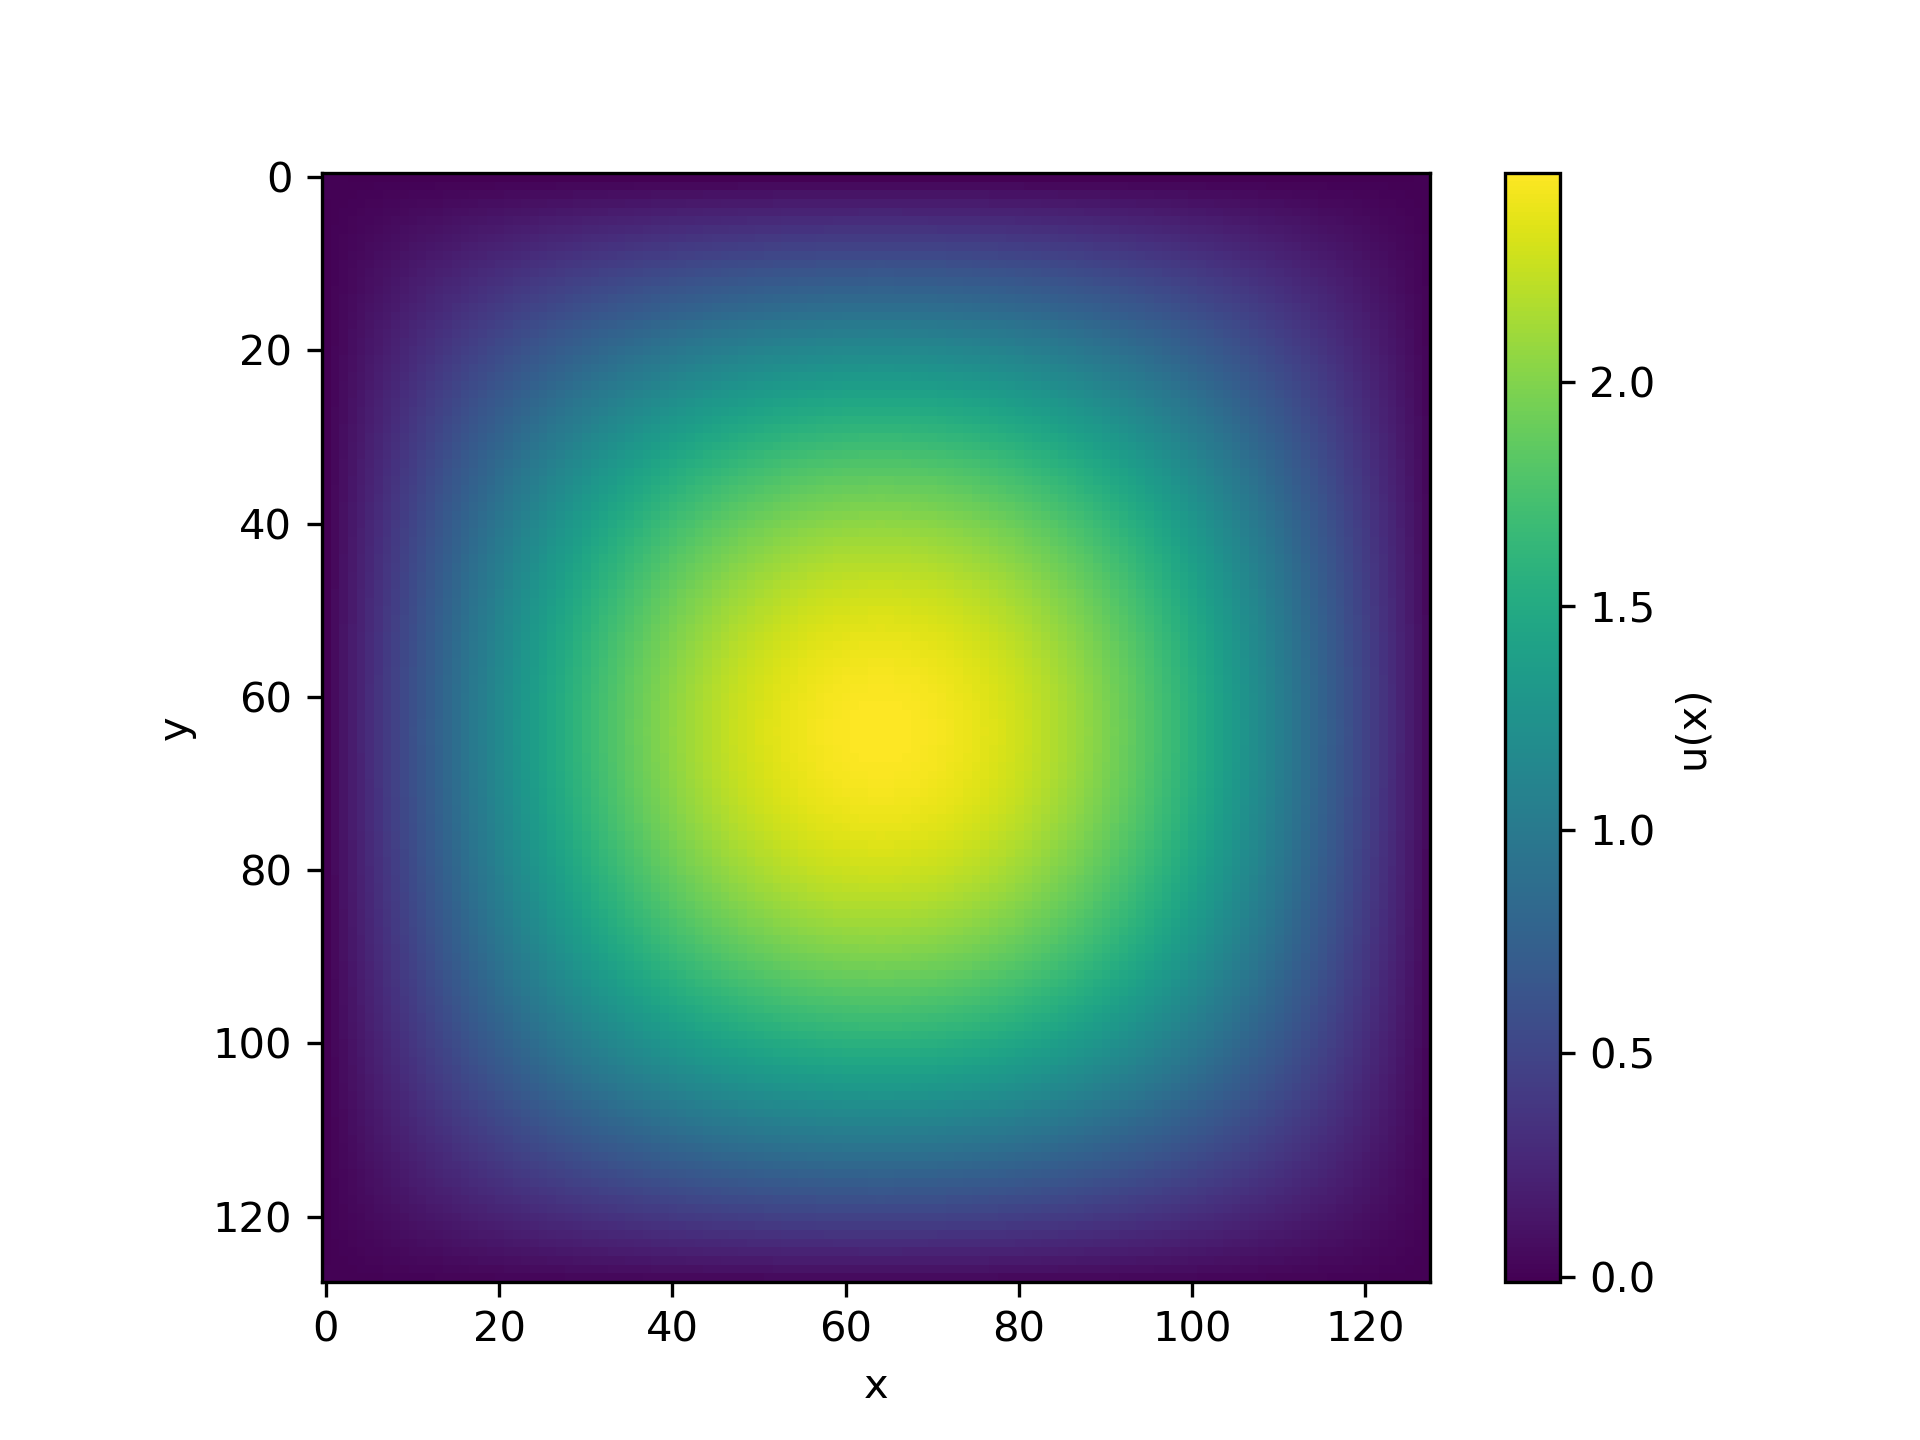
\includegraphics[width=.6\linewidth]{./q2plot.png}
        \caption{}
        \label{fig:q2_fig}
    \end{figure}	


\section*{3.3}
	
	In figure 2 chose to plot a semilogx plot. I plotted the error bound given in 
	the question in dotted line and the actual error I computed, assuming the true 
	solution to the problem is the final step in the iteration. In my plot you can see
	that my error is not exactly bound by the error bound in later iterations. The 
	curves do however look like a bit like a scaled version of the bounding functions,
	following a vaguely similar scaled trajectory. What is good is that the error 
	decreases as the number of iterations increases.
	
	\begin{figure}[h!]
        \centering
        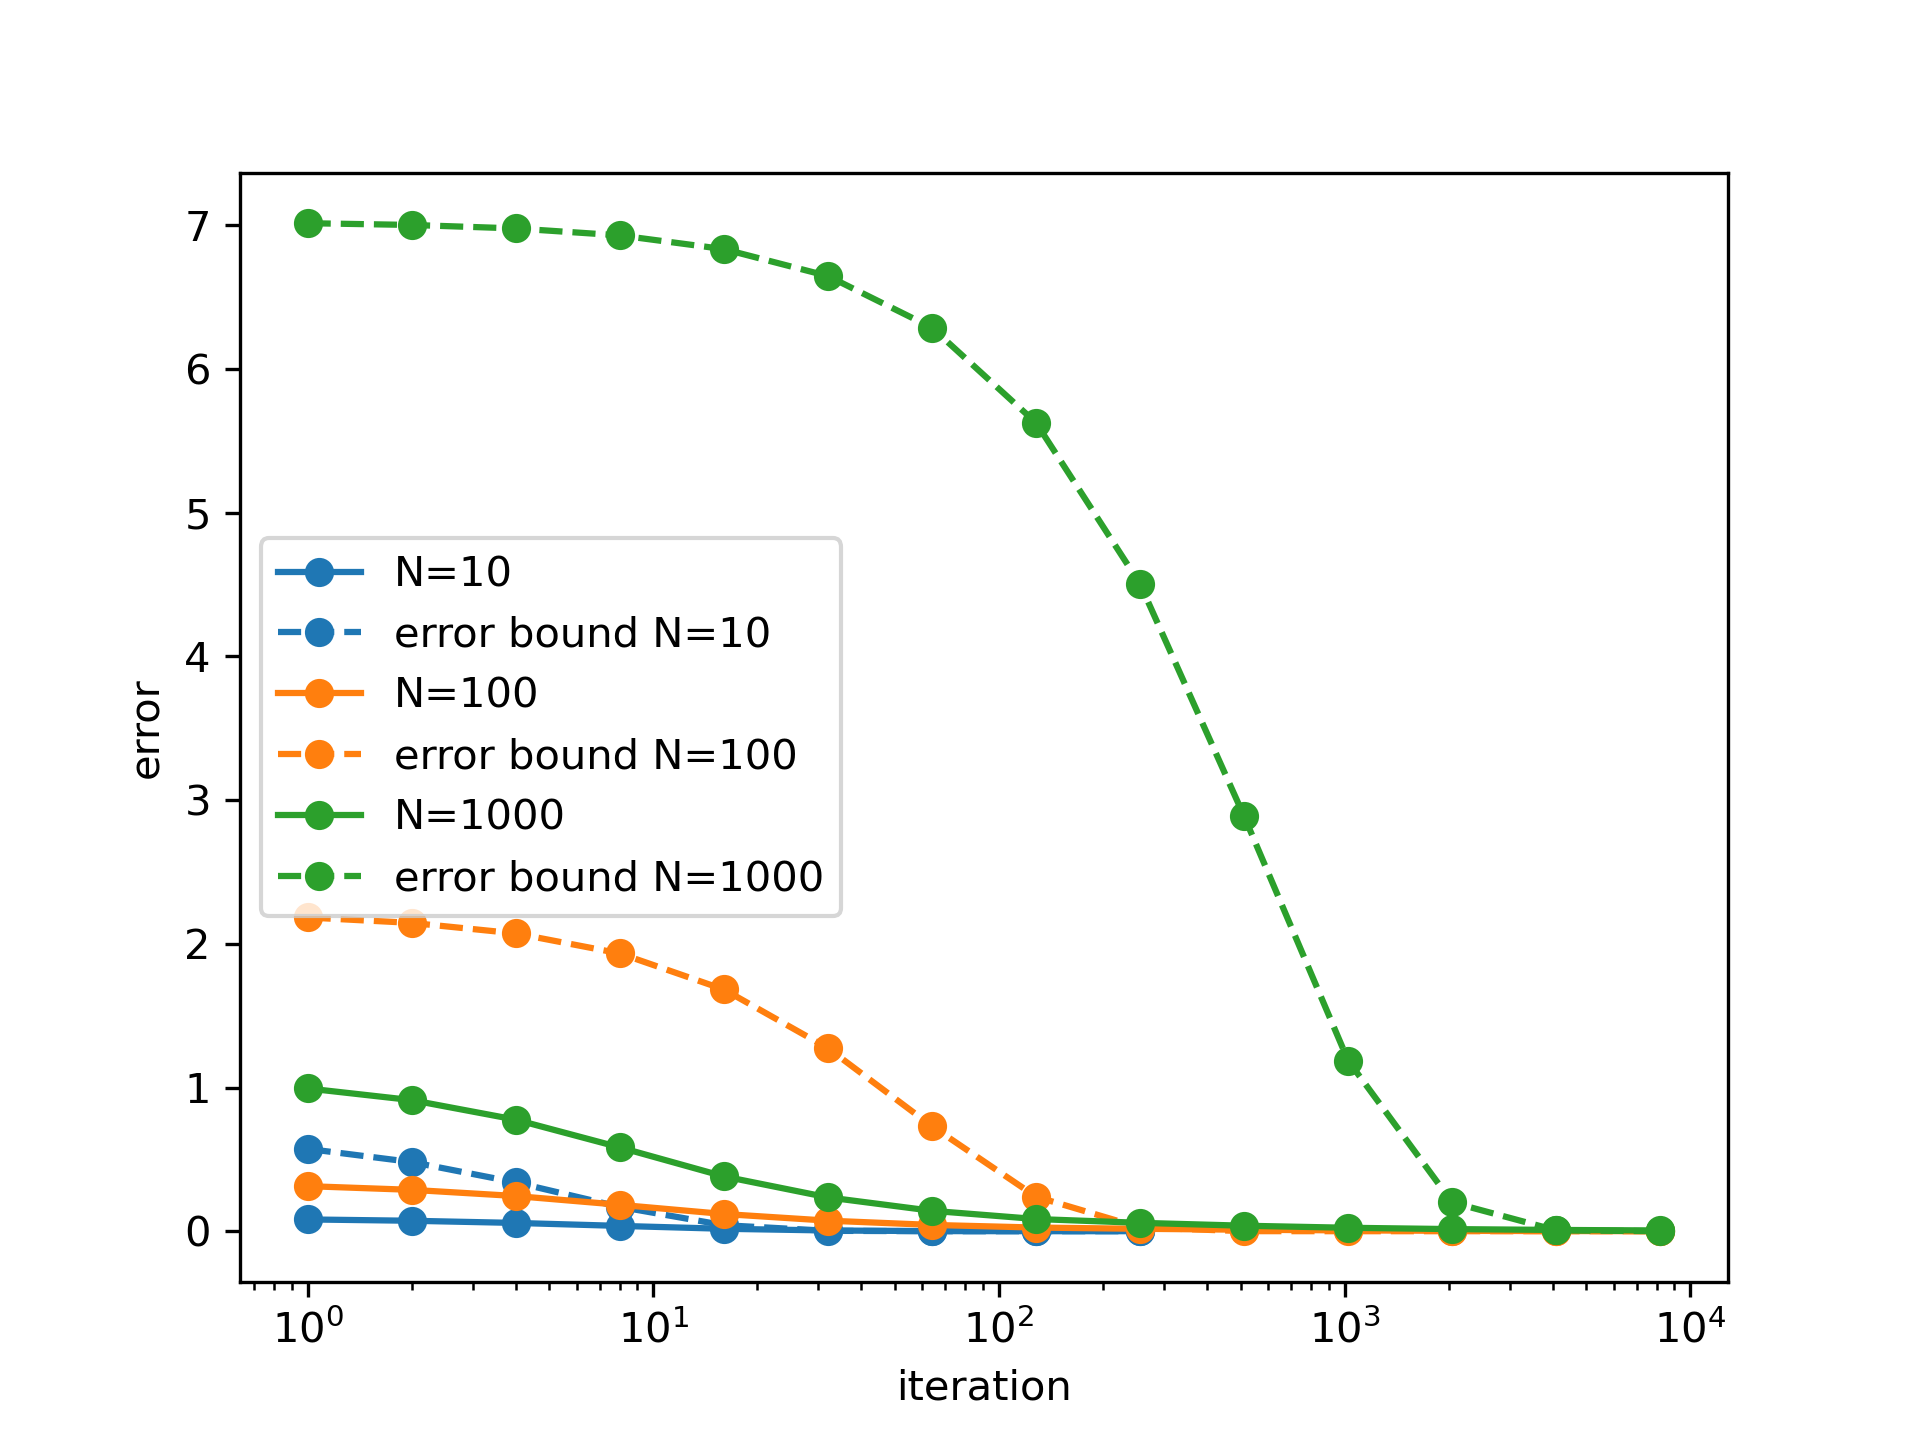
\includegraphics[width=.6\linewidth]{./q3plot.png}
        \caption{}
        \label{fig:q2_fig}
    \end{figure}	

\end{document}
